For CE development, testing prototypes at room temperature is the first step, as many problems can be identified quickly and without the expense of cryogens.  A quick access test stand with the FEMB connected to an APA inside a shielded environment that is in the same location as the FEMB/ASIC development is invaluable for rapid progress.  Two such facilities are available to DUNE: the shielded room at Fermilab and the 40\% APA test stand at BNL.  In addition, a ``cold box'' at CERN used in electronics tests for ProtoDUNE-SP is available for additional electronics testing in cold argon gas.

The shielded room at Fermilab (see Figure~\ref{fig:shieldedroom}) is 2.5~m tall, and 2~m on each side, with 
a double layer of copper mesh in the walls, floor and ceiling, plus a solid metal plate in the floor all electrically connected to create a faraday cage.  A flexible AC distribution and isolated grounding configuration offers the ability to easily ground the shielded room and power the associated electronics from either a building reference or a detector reference.  In addition
to evaluating different grounding schemes for the APAs, capacitive coupling issues can be studied by varying the
distance between the floor and a copper plate positioned underneath.   
This room has uniquely easy access to the setup through a shielded door,
and a person can remain inside safely with the door closed and probe the electronics directly while operating
in a shielded environment.  Currently mounted inside are two 35-ton APAs 
with adaptor boards to connect ProtoDUNE electronics.  This installation satisfies the ProtoDUNE grounding and shielding guidelines.  A rough demonstration of the shielding adequacy for our purposes  is the measured noise level of 800~ENC for ProtoDUNE prototype FEMBs.  The same noise level was measured at room temperature in the 40\% APA at BNL for the same FEMBs.

\begin{dunefigure}
[Picture of the shielded room at Fermilab.]
{fig:shieldedroom}
{Picture of the shielded room at Fermilab.}
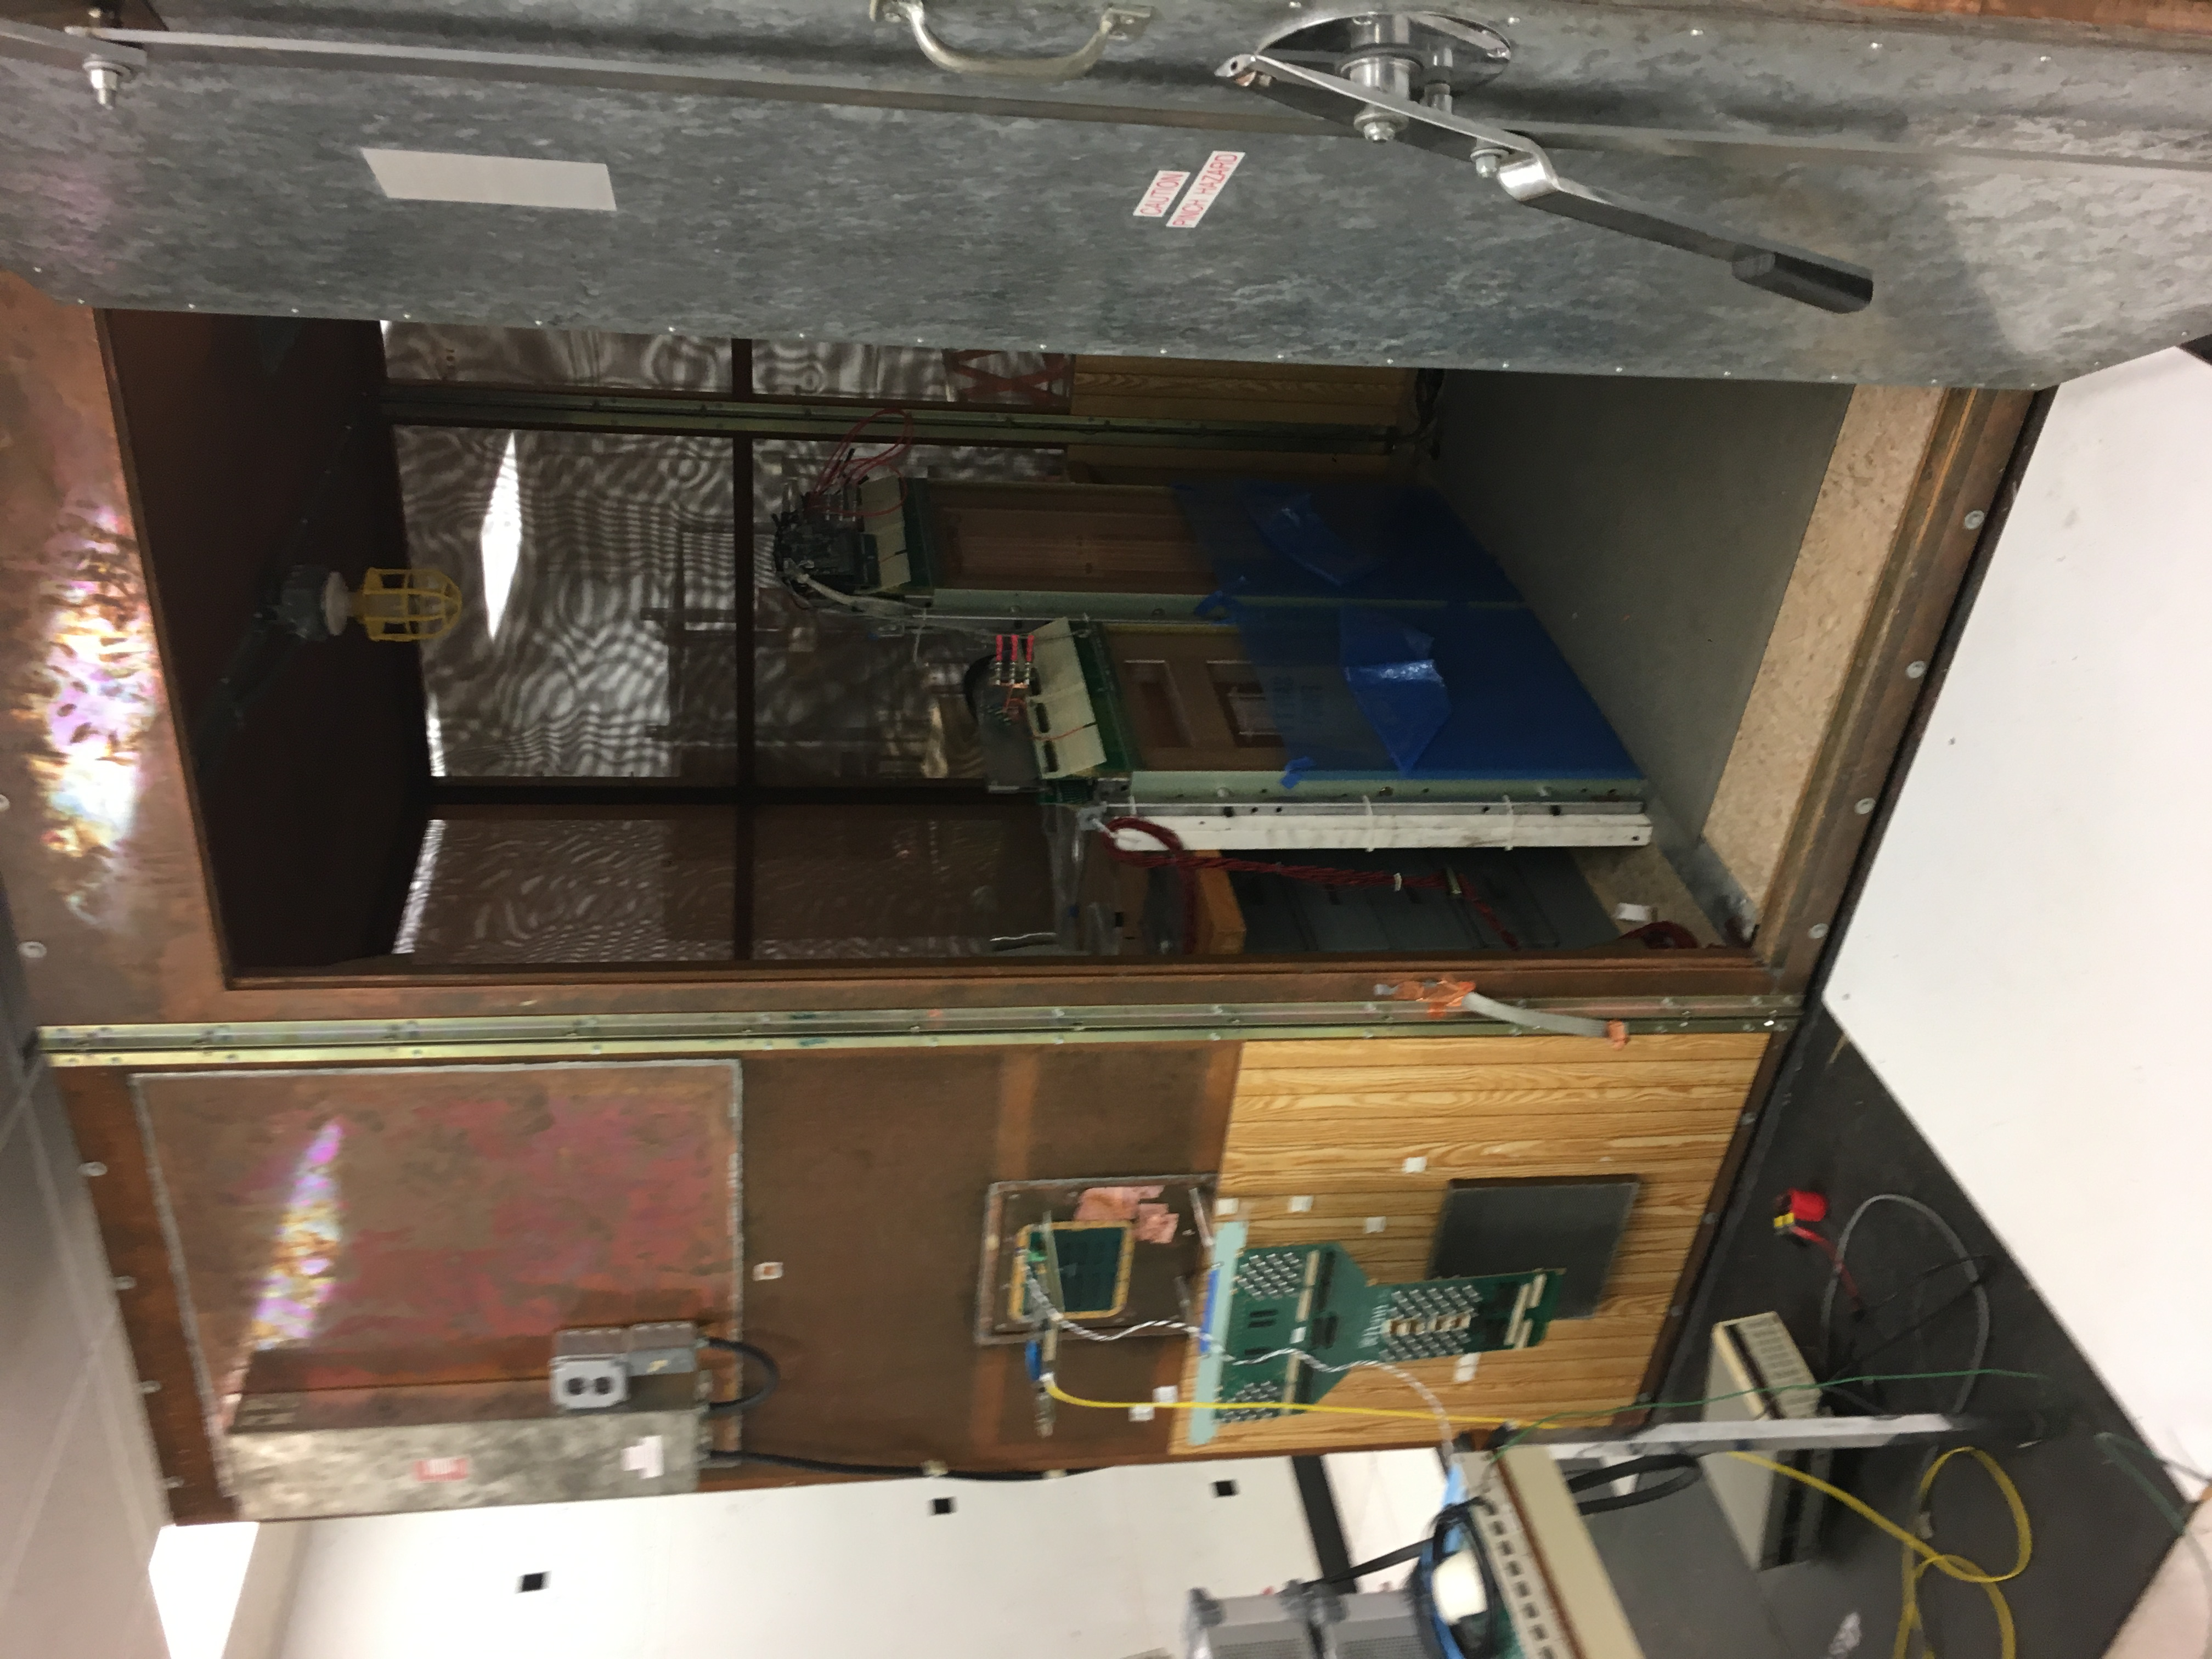
\includegraphics[angle=270,width=0.4\linewidth]{tpcelec-shielded_room.jpg}
\end{dunefigure}

The 40\% APA at BNL is a 2.8~m~$\times$~1.0~m three-plane APA with two layers of 576 wrapped (U/V) wires and one layer of 448 straight (X) wires. It is read out by 8 ProtoDUNE-SP FEMBs with the full 7~m ProtoDUNE-SP length data and LV power cables, 4 on the top and 4 on the bottom. Its readout uses the full CE system for ProtoDUNE-SP, with a prototype CE flange and WIEC, 2 WIBs and 1 PTC, as shown in Figure~\ref{fig:tpcelec_40APA}. Detailed integration tests of the CE readout performance while following the DUNE grounding and shielding guidelines have been done at the 40\% APA. Additional input capacitance (equivalent to longer wire length) have been added to a subset of channels to project the ENC performance from the 40\% APA teststand to the ProtoDUNE-SP and SBND detectors. The results from the 40\% APA indicate that the full CE system as installed on the teststand at BNL will satisfy the DUNE far detector noise requirements.

\begin{dunefigure}
[Left: one side of the 40\% APA with 4 FEMBs.  Right: the full CE feedthrough and flange.]
{fig:tpcelec_40APA}
{Left: one side of the 40\% APA with 4 FEMBs.  Right: the full CE feedthrough and flange.}
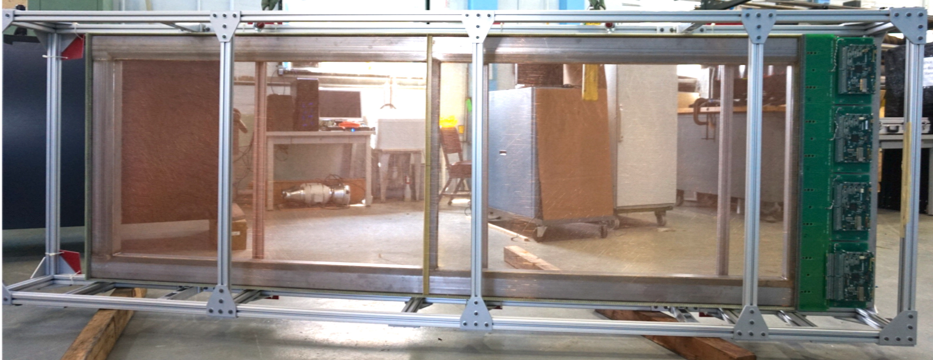
\includegraphics[width=0.72\linewidth]{tpcelec-40-apa.png}
\hspace{3mm}
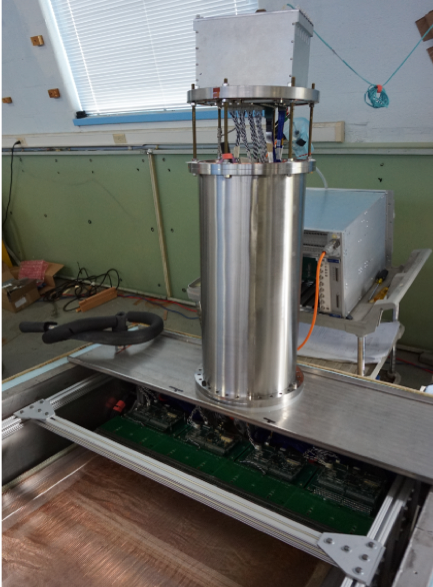
\includegraphics[width=0.2\linewidth]{tpcelec-40-apa-ft.png}
\end{dunefigure}

%\begin{figure}
%    \centering
%    \includegraphics[width=0.9\linewidth]{tpcelec-40-apa-result.png}
%    \caption{ENC (in electrons) as a function of input capacitance (equivalent to input wire length) measured on the 40\% APA. The ENC projections are based on the input wire length of the SBND and ProtoDUNE-SP detectors.}
%    \label{fig:tpcelec_40APA_results}
%\end{figure}

The cold box at CERN is designed to cycle one full-size DUNE APA with the full compliment of 20 FEMB through gaseous Nitrogen temperatures around 150K to check out the APA performance prior to installing the APA into the ProtoDUNE-SP cryostat. It is designed to be a Faraday cage identical to the ProtoDUNE-SP cryostat and is read out by a complete CE system for a single APA, including a CE flange and fully-loaded WIEC with 5 WIBs and 1 PTC.
